\subsection{A 25. napciklus előrejelzése}

\begin{frame}{}
    \centering
    \Huge{A 25. napciklus előrejelzése}\\
    \vspace*{1cm}
    \large{Benson, B., Pan, W.D., Prasad, A. et al. \\ \href{https://arxiv.org/pdf/2005.12406.pdf}{Forecasting Solar Cycle 25 Using Deep Neural Networks}. \\ Sol Phys 295, 65 (2020)}
\end{frame}

\begin{frame}{Napciklus}
    \centering
    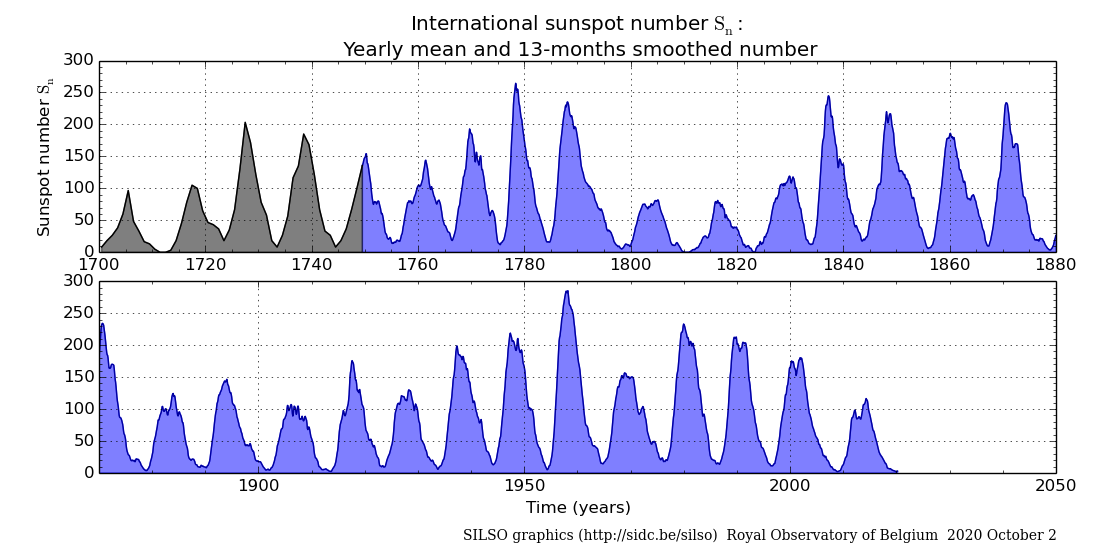
\includegraphics[width=1.0\textwidth]{figures/sunspot_number.png}
\end{frame}

\begin{frame}{Előrejelzés mozgó átlaggal}
    \begin{itemize}
        \item Minimális ablak: 2 ciklus (= 1 mágneses ciklus), de:
    \end{itemize}
    \centering
    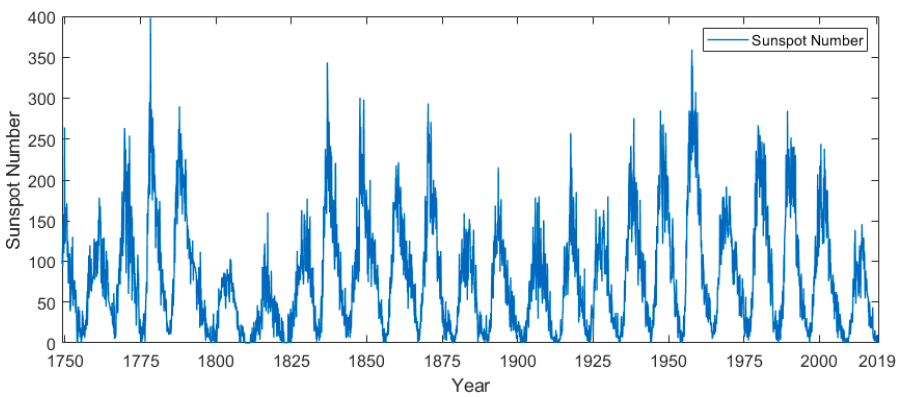
\includegraphics[width=0.5\textwidth]{figures/solar_cycle_zoom.png}
    
    \pause
    \begin{itemize}
        \item Pontosabb előrejelzés: 4 ciklus hosszú ablak, egy ciklus hosszú előrejelzés, de:
    \end{itemize}
    \centering
    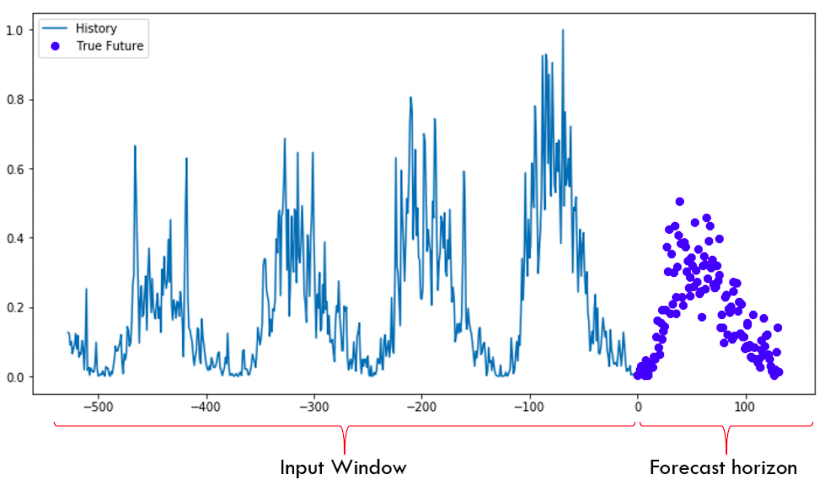
\includegraphics[width=0.45\textwidth]{figures/solar_cycle_moving_avg.png}
\end{frame}

\begin{frame}{Long Short Term Memory (LSTM) hálózatok}
    \href{https://colah.github.io/posts/2015-08-Understanding-LSTMs/}{Understanding LSTM Networks (colah's blog)}
    
    Recurrent Neural Network (RNN):
    
    \centering
    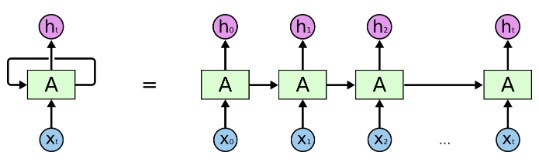
\includegraphics[width=0.7\textwidth]{figures/rnn.png} \\ \footnotesize{colah's blog}
    
    \normalsize
    \begin{itemize}
        \item Képes régi dolgokra "visszaemlékezni"
        \item Gyakorlatban nem, csak a rövidtávú dolgokra ("rövidtávú memóriája van")
    \end{itemize}
\end{frame}

\begin{frame}{Long Short Term Memory (LSTM) hálózatok}
    \href{http://www.bioinf.jku.at/publications/older/2604.pdf}{Hochreiter \& Schmidhuber (1997)} \\
    
    RRN modul:\\
    \centering
    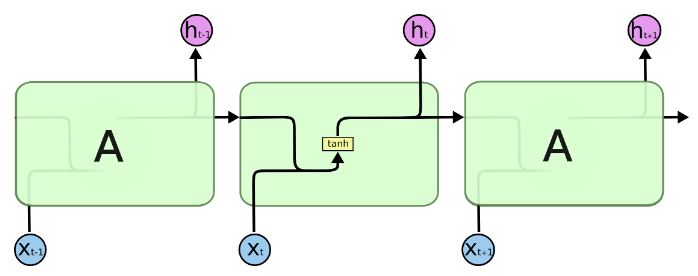
\includegraphics[width=0.65\textwidth]{figures/lstm_only_rnn.png}
    
    \raggedright LSTM modul: \\
    \centering
    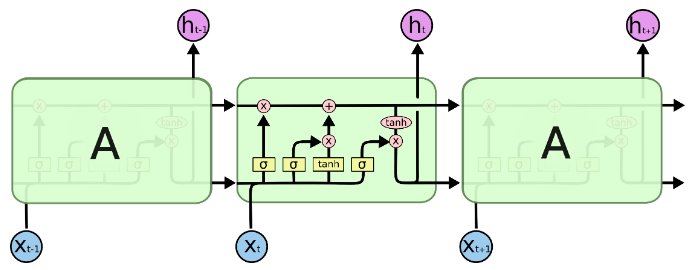
\includegraphics[width=0.65\textwidth]{figures/lstm_module.png}
\end{frame}

\begin{frame}{WaveNet}
    \href{https://deepmind.com/blog/article/wavenet-generative-model-raw-audio}{WaveNet} - generatív modell hang generáláshoz
    \centering
    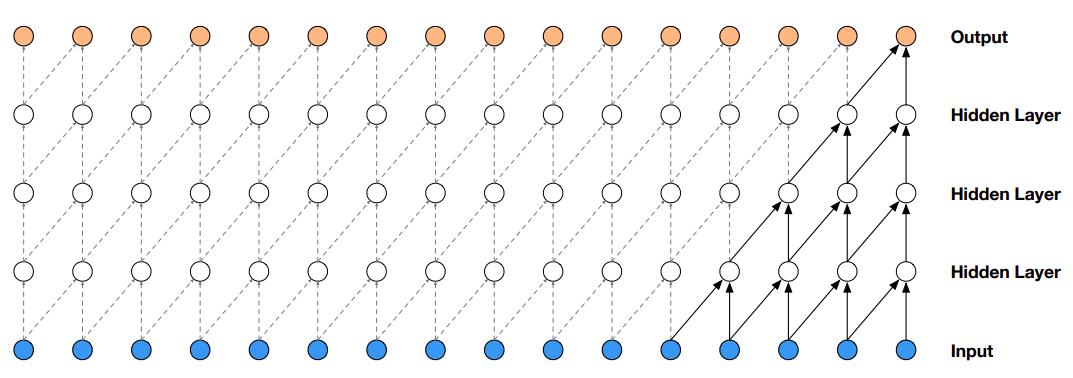
\includegraphics[width=1.0\textwidth]{figures/wavenet_casual_cnn.png}
\end{frame}

\begin{frame}{WaveNet}
    \href{https://deepmind.com/blog/article/wavenet-generative-model-raw-audio}{WaveNet} - generatív modell hang generáláshoz
    \centering
    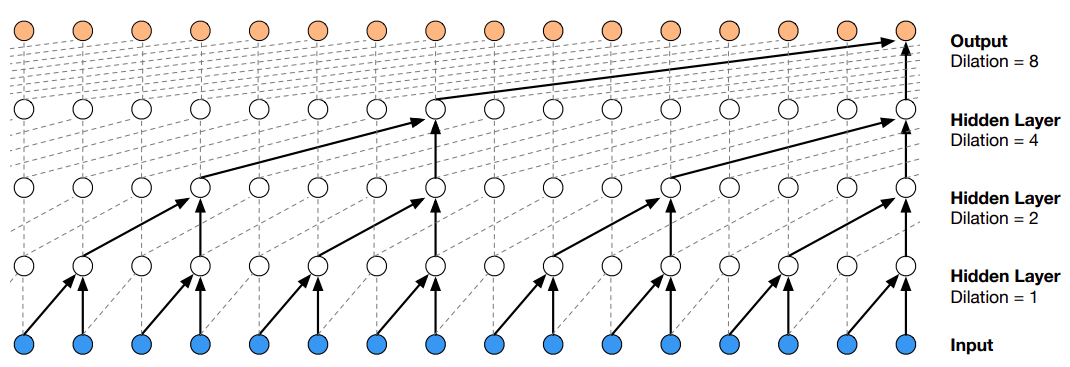
\includegraphics[width=1.0\textwidth]{figures/wavenet_dilated_cnn.png}
\end{frame}

\begin{frame}{Az alkalmazott modell}
    \centering
    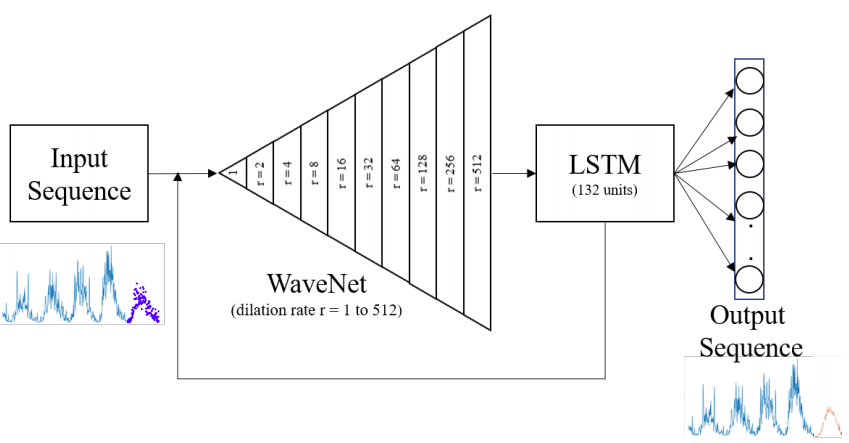
\includegraphics[width=1.0\textwidth]{figures/solar_cycle_model.png}
\end{frame}

\begin{frame}{Miért?}
    \begin{itemize}
        \item Klasszikus előrejelző módszerek lineáris összefüggést és ismert eloszlást feltételeznek
        \item LSTM nem feltételez semmit a rövid- és hosszútávú változásról
        \item Bonyolult, nemlineáris rendszerek is modellezhetők
        \item Generatív modellekkel tovább erősíthető (pl. WaveNet)
    \end{itemize}
\end{frame}

\begin{frame}{Két modell összehasonlítása - Két LSTM}
    \centering
    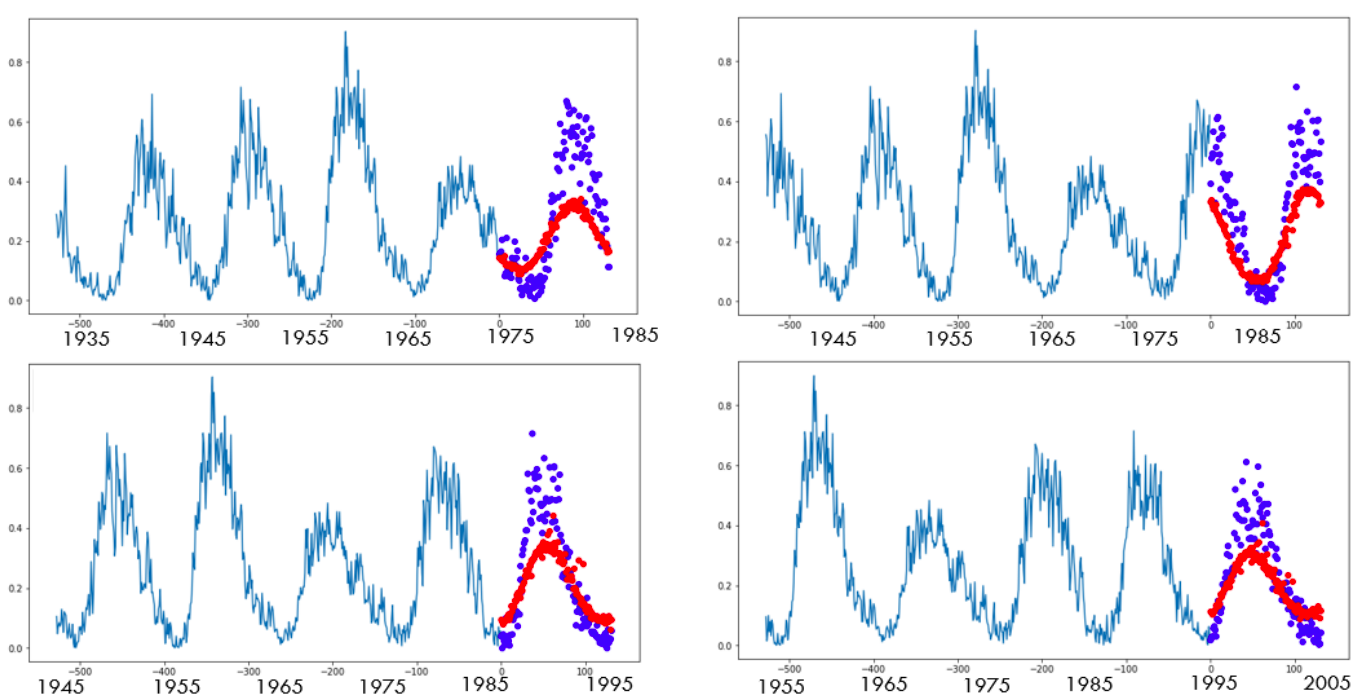
\includegraphics[width=1.0\textwidth]{figures/solar_cycle_stacked_lstm.png}
\end{frame}

\begin{frame}{Két modell összehasonlítása - WaveNet + LSTM}
    \centering
    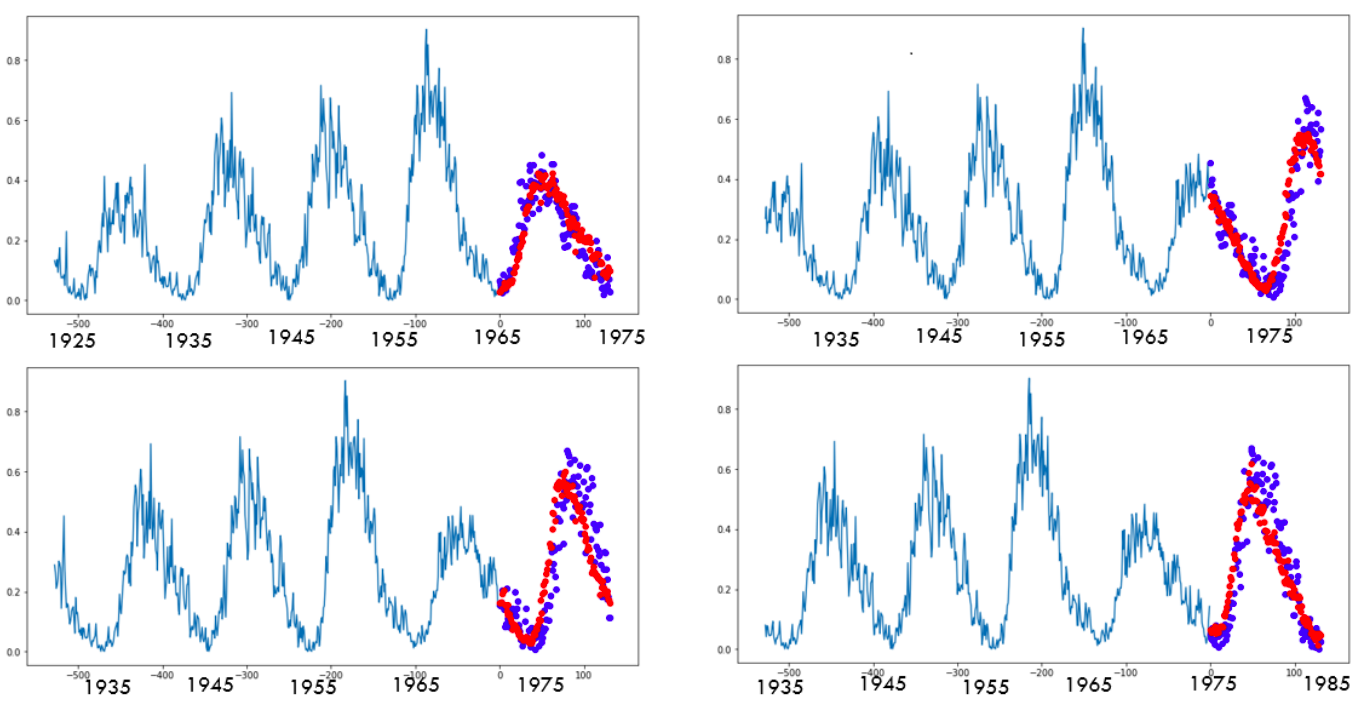
\includegraphics[width=1.0\textwidth]{figures/solar_cycle_wavenet_lstm.png}
\end{frame}

\begin{frame}{Az előrejelzés}
    \centering
    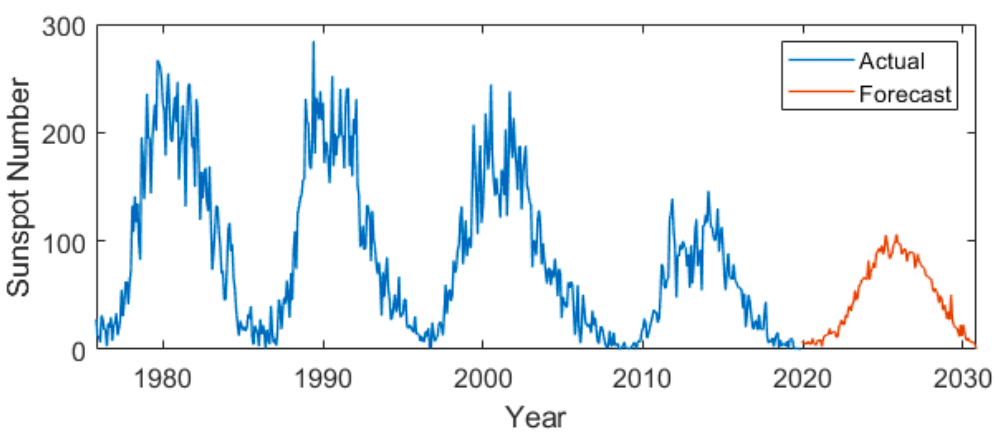
\includegraphics[width=1.0\textwidth]{figures/forecasting_solar_cycle.png}
    \begin{itemize}
        \item Napfoltszám max: $106 \pm 19.75$
        \item Maximum: 2025 március
    \end{itemize}
\end{frame}